\documentclass[a4paper, 12pt]{article}
\usepackage{a4wide}
\usepackage {amsmath}
\usepackage{amssymb}
\usepackage {graphicx}
\usepackage[utf8]{inputenc} 
\usepackage[francais]{babel}
\usepackage{fancyhdr}
\usepackage{setspace}
\usepackage{fancyhdr}
\usepackage{lastpage}
\usepackage{extramarks}
\usepackage{chngpage}
\usepackage{soul}
\usepackage{algorithmicx} 
\usepackage{algpseudocode} 
\usepackage{multicol}
\usepackage[usenames,dvipsnames]{color}
\usepackage{graphicx,float,wrapfig}
\usepackage{ifthen}
\usepackage{listings}
\usepackage{courier}
\usepackage{esint}
\usepackage{bbm}
\usepackage{graphics}
\usepackage{graphicx}
\usepackage{subfig}
\usepackage{epsfig}
\usepackage{pgf,tikz}
\usetikzlibrary{arrows}
\usepackage{braket}
\usepackage{MnSymbol,wasysym}
\usepackage{marvosym}
\usepackage{dsfont}
\usepackage{listings}
\usepackage{color}

\definecolor{mygreen}{rgb}{0,0.6,0}
\definecolor{mygray}{rgb}{0.5,0.5,0.5}
\definecolor{mymauve}{rgb}{0.58,0,0.82}

\lstset{ %
  backgroundcolor=\color{white},   % choose the background color; you must add \usepackage{color} or \usepackage{xcolor}; should come as last argument
  basicstyle=\footnotesize,        % the size of the fonts that are used for the code
  breakatwhitespace=false,         % sets if automatic breaks should only happen at whitespace
  breaklines=true,                 % sets automatic line breaking
  captionpos=b,                    % sets the caption-position to bottom
  commentstyle=\color{mygreen},    % comment style
  deletekeywords={...},            % if you want to delete keywords from the given language
  escapeinside={\%*}{*)},          % if you want to add LaTeX within your code
  extendedchars=true,              % lets you use non-ASCII characters; for 8-bits encodings only, does not work with UTF-8
  frame=single,	                   % adds a frame around the code
  keepspaces=true,                 % keeps spaces in text, useful for keeping indentation of code (possibly needs columns=flexible)
  keywordstyle=\color{blue},       % keyword style
  language=Python,                 % the language of the code
  morekeywords={*,...},           % if you want to add more keywords to the set
  numbers=left,                    % where to put the line-numbers; possible values are (none, left, right)
  numbersep=5pt,                   % how far the line-numbers are from the code
  numberstyle=\tiny\color{mygray}, % the style that is used for the line-numbers
  rulecolor=\color{black},         % if not set, the frame-color may be changed on line-breaks within not-black text (e.g. comments (green here))
  showspaces=false,                % show spaces everywhere adding particular underscores; it overrides 'showstringspaces'
  showstringspaces=false,          % underline spaces within strings only
  showtabs=false,                  % show tabs within strings adding particular underscores
  stepnumber=1,                    % the step between two line-numbers. If it's 1, each line will be numbered
  stringstyle=\color{mymauve},     % string literal style
  tabsize=2,	                   % sets default tabsize to 2 spaces
  title=\lstname                   % show the filename of files included with \lstinputlisting; also try caption instead of title
}

\newtheorem{de}{Définition}[subsection] % les definitions et les theoremes sont
\newtheorem{theo}{Theoreme}[section]    % numerotes par section
\newtheorem{prop}[theo]{Proposition}    % Les propositions ont le meme compteur
                                        % que les theoremes

\DeclareMathOperator{\tr}{tr}

\lhead{} 
\chead{} 
\rhead{\bfseries Python} 
\lfoot{J.-C. Toussaint & L. Bastard - Phelma }
%\cfoot{} 
%\rfoot{\thepage}

% Includes a MATLAB script.
% The first parameter is the label, which also is the name of the script
%   without the .m.
% The second parameter is the optional caption.
\newcommand{\matlabscript}[2]
  {\begin{itemize}\item[]\lstinputlisting[caption=#2,label=#1]{#1.m}\end{itemize}}

\lhead{} 
\chead{} 
\rhead{\bfseries Python} 
\lfoot{JC Toussaint - Phelma }

\pagestyle{fancy}

\begin{document}

\bibliographystyle{alpha}

\title{Le projet : le chiffrement de César}

\author{Jean-Christophe Toussaint \& Lionel Bastard \\
%  Phelma\\
 \texttt{prenom.nom@phelma.grenoble-inp.fr}}
\date{\today}
 
\maketitle

 \fbox{\parbox{\textwidth}{
Le rendu sera sous la forme d'un fichier unique python où 
les réponses seront insérées sous la forme de commentaires.
On vous conseille d'utiliser l'environnement Jupyter pour développer votre programme python.

%Le sous-répertoire {\bf pcode} contient une version fonctionnelle mais non lisible de ce projet.
%Les fonctions Matlab sont en version compilée et portent le suffixe {\bf.p}
%
%Si vous n’arrivez pas à développer une fonction Matlab, copier sa version compilée .p dans votre répertoire {\bf src} pour continuer le développement du projet. {\bf Elle est appelée en priorité par Matlab}. Supprimez-la ensuite de votre répertoire {\bf src}  pour tester votre propre fonction.

}}

%L'exercice, proposé ci-après, est à réaliser en totale autonomie et constitue le socle
%de base en Python que vous devez assimiler.

\section{Principe}

En cryptographie, le chiffrement de César, également appelé chiffrement de César, chiffrement par décalage, code de César ou décalage de César, est l'une des techniques de chiffrement les plus simples et les plus connues. Il s'agit d'un type de chiffrement par substitution dans lequel chaque lettre du texte en clair est remplacée par une lettre située à un nombre fixe de positions dans l'alphabet. Par exemple, avec un décalage vers la gauche de 3, D est remplacé par A, E devient B, et ainsi de suite. La méthode doit son nom à Jules César, qui l'utilisait dans sa correspondance privée.

\begin{figure}[h!]
\centering
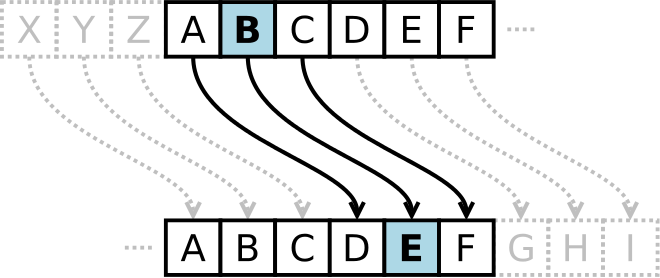
\includegraphics[scale=0.3]{660px-Caesar3.png}
\caption{Le chiffre de César fonctionne par décalage des lettres de l'alphabet. Source wikipedia.}
\label{cesar}
\end{figure}

L'étape de chiffrement effectuée par un chiffrement de César est souvent incorporée dans des schémas plus complexes, tels que le chiffrement de Vigenère, et a encore une application moderne dans le système ROT13. Comme tous les chiffres de substitution à un seul alphabet, le chiffre César est facilement cassé et, dans la pratique moderne, n'offre pratiquement aucune sécurité de communication. 

\section{Préambule}

On donne ci-après quelques instructions de base python pour réaliser votre projet.

\begin{enumerate} 
\item La fonction membre {\tt index(element)} de la classe list, donne la position de la première occurence d'un élément rencontré dans une liste.

Exemple : soit  abc=['A', 'B', 'C', 'D', 'E'],  abc.index('A') retourne 0,  abc.index('E') retourne 4, tandis que abc.index('Z') génère
une erreur du type  « ValueError » car 'Z' n'est pas un élément de la liste.

\item La fonction python {\tt chr(n)} renvoie le caractère associé au code ASCII $n \in [0, 128[$. Elle prend un seul entier comme argument.
 Si l’entier passé en paramètre est en dehors de la plage, la méthode retourne « ValueError ».
 Exemple : chr(65) retourne 'A'.

\item La fonction python {\tt ord(c)} renvoie la valeur ASCII associé au caractère c. Si la longueur de la chaîne passée en paramètre est supérieure à un, une erreur « TypeError » est générée. Exemple : ord('A') retourne 65.

\item La fonction membre upper() de la classe string permet de transformer une chaine comportant des caractères minuscules en majuscules.
Exemple ''aBc''.upper() retourne ''ABC''.

\item L'astuce suivante permet de  transformer une liste de caractères en une chaine de caractères : ''.join(['A', 'B', 'C']) où '' est le caractère vide (2 fois simple quote) retourne la chaine ''ABC''.  
\end{enumerate}

\section{Exercices}

\begin{enumerate} 
\item Générer la liste abc contenant les caractères allant de 'A' jusqu'à 'Z'. Ajouter-lui à droite le caractère blanc. 

\item Générer la liste abc\_cipher à partir de la liste précédente abc, décalé d'un entier shift. Avec shift=3, vous devez retrouver le résultat de la figure
\ref{cesar}.

\end{enumerate} 

\section{Développement}

\begin{enumerate} 
\item Dévélopper une fonction {\tt encrypt\_string(string, shift)} qui à partir d'une chaine de caractères string
retourne sa version cryptée pour un décalage fixé shift.

\item Dévélopper une fonction {\tt  decrypt\_string(string, shift)} qui fait l'opération inverse.

\item Dévélopper un programme principal, permettant de valider les deux fonctions précédentes, en prenant quelques exemples.
N'oubliez pas de transformer la chaine de caractères saisie en sa version en majuscules avant de l'encrypter.
Quelles limitations identifiez-vous?

\end{enumerate} 

\section{Application à un document texte}

On vous demande de développer une version plus élaborée qui fera le cryptage d'un texte contenu dans un fichier texte.

\begin{enumerate} 
\item Dévélopper d'abord une fonction {\tt readfile(filename)} qui lit le texte au format ASCII depuis le fichier de nom filename
et qui retourne une liste contenant chaque ligne du fichier sous la forme d'un élément de liste. 
Cette liste sera nommé {\tt page}.

\noindent {\it Indication :} on utilisera la fonction readlines().

\item Développer une fonction {\tt encrypt\_page} qui encrypte la liste précédente {\tt page} en fixant le décalage shift à 3. 
Elle retournera la liste des lignes cryptées.
Pour éliminer le caractère de fin de ligne '\textbackslash n', on appliquera la fonction membre {\tt rstrip('\textbackslash n')} à chaque ligne lue.

\item Dévélopper une fonction {\tt decrypt\_page} permettant de décrypter une liste cryptée de chaines de caractères.
La valeur de shift est fixée à 3.

\item Développer une fonction {\tt savefile(filename, page) } pour sauvegarder cette liste encryptée dans un fichier 
dont le radical est celui d'origine complété par le suffixe ''\_cipher''.
page est une liste de chaines de caractères en majuscule.

\noindent Par exemple : si filename est ''OnlyForYourEyes.txt'' alors le nom du fichier crypté s'appelera ''OnlyForYourEyes\_cipher.txt''.

{\it Indication :} utiliser la fonction membre split('.') de la classe string pour découper le nom du fichier en utilisant le séparateur '.'



\end{enumerate} 



\end{document}

